\documentclass[11pt]{article}
\usepackage[margin=1in]{geometry}
\usepackage{graphicx,booktabs,amsmath,siunitx,caption,xcolor,enumitem}
\usepackage[hidelinks]{hyperref}
\usepackage{natbib}
\usepackage{titlesec}
\titleformat{\section}{\large\bfseries}{\thesection}{0.6em}{}
\titleformat{\subsection}{\normalsize\bfseries}{\thesubsection}{0.6em}{}
\setlength{\parskip}{0.4em}\setlength{\parindent}{0pt}
\captionsetup{font=small,labelfont=bf}
\graphicspath{{figures/}}\sisetup{group-separator={,}}

\title{\bfseries A Value-at-Risk and Hedging Framework for Henry Hub Natural Gas:\\
GARCH Core with a Machine-Learning Volatility-Regime Layer}
\author{}\date{August 2026}
\begin{document}\maketitle\vspace{-2.5em}

\begin{abstract}\noindent
We build a Value-at-Risk (VaR) and hedging analysis for Henry Hub natural-gas
exposure using the standard risk-desk toolkit---a GARCH(1,1) volatility model with
a Student-$t$ innovation, VaR by parametric, historical and GARCH methods, Kupiec
coverage backtesting, and a minimum-variance CME futures hedge---and add a
machine-learning (ML) layer targeted at the one thing GARCH does poorly: detecting
volatility-regime shifts. A Gaussian Hidden Markov Model and a gradient-boosting
classifier, informed by heating/cooling degree days and storage deviations,
identify the stressed regime better than a GARCH-threshold rule (AUC
\num{0.90}/\num{0.86} vs \num{0.84}) and flag \SI{69}{\percent} of regime onsets
pre-emptively versus GARCH's \SI{39}{\percent}, about a day earlier on average.
Feeding this into a regime-aware VaR cuts \SI{99}{\percent} breaches from 29 to 16
on a \num{2264}-day sample and removes breach \emph{clustering} (at most one breach
in any ten-day window, versus three for GARCH). A minimum-variance hedge of roughly
\num{430} CME NG contracts reduces the \SI{99}{\percent} VaR of a hypothetical
\SI{5}{} million-MMBtu long position by \SI{56.7}{\percent}, and a
regime-conditional dynamic hedge lowers deep-tail expected shortfall a further
\SI{\sim9}{\percent}. Because natural gas is the primary dispatchable bridge fuel
backing new electricity capacity amid surging data-center demand, regime-aware gas
risk management is a direct input to grid-cost reliability. \emph{Data note:} the
in-repository price path is a reproducible simulation calibrated to real EIA
published statistics and documented volatility episodes (the methodology and code
run unchanged on the live EIA/NOAA series); this is disclosed in \S\ref{sec:data}.
\end{abstract}

\section{Motivation}
Natural gas sets the marginal price of electricity across most U.S. hours and is the
dispatchable backbone against which intermittent renewables and surging
data-center load are balanced. Henry Hub is also one of the most volatile
commodities traded: the spot price ran from an all-time monthly low of
\SI{1.51}{\$/MMBtu} in March 2024 \citep{eia_hh_2024low} to a \SI{9.86}{\$/MMBtu}
daily high in January 2025 \citep{eia_hh_2025}, with the February 2021 Winter Storm
Uri event driving record daily spikes. Annual averages swung from
\SI{6.45}{\$/MMBtu} (2022) to \SI{2.57}{} (2023), \SI{2.21}{} (2024, a record low),
and back to \SI{3.52}{} (2025) \citep{eia_hh_2023,eia_hh_2024low,eia_hh_2025}, with
EIA projecting \SI{\sim3.50}{} in 2026 and \SI{\sim4.60}{} in 2027 as LNG exports
tighten the balance \citep{eia_steo_2026}. An energy company with physical gas
exposure needs (i) an accurate, responsive measure of tail risk and (ii) a hedge
that reduces it. The risk desk's standard answer is GARCH-based VaR plus a futures
hedge; our contribution is to show where a targeted ML layer measurably improves it.

\section{Data and Sources}\label{sec:data}
Primary/official sources only: EIA (Henry Hub spot and weekly storage), NOAA
(heating/cooling degree days), and CME Group (the NG futures contract
specification). Table~\ref{tab:p2src} lists them; full provenance, URLs and access
dates are in the repository's \texttt{data/SOURCES.md}.

\begin{table}[h]\centering\small
\caption{Primary sources (access date 2026-08-19).}\label{tab:p2src}
\begin{tabular}{@{}p{4.6cm}p{4.2cm}p{5.2cm}@{}}\toprule
\textbf{Series} & \textbf{Source} & \textbf{Use}\\\midrule
Henry Hub annual/daily spot & EIA Today-in-Energy \citep{eia_hh_2025,eia_hh_2024low,eia_hh_2023} & Calibration anchors, price level\\
Price forecast, LNG, storage & EIA STEO \citep{eia_steo_2026} & Forward context\\
Weekly working-gas storage & EIA \citep{eia_ng_storage} & Demand/supply driver (feature)\\
Heating/cooling degree days & NOAA CPC \citep{noaa_degree_days} & Weather demand driver (feature)\\
NG futures contract spec & CME Rulebook Ch.~220 \citep{cme_ng_specs} & Hedge instrument definition\\
\bottomrule\end{tabular}\end{table}

\paragraph{Data mode and honesty disclosure.} The environment used to assemble this
study cannot download the live bulk price history. The working series is therefore
a \textbf{reproducible, seed-fixed, regime-switching simulation of the daily Henry
Hub spot price, calibrated to the real EIA annual averages above and to documented
volatility episodes} (COVID-2020 lows, Winter Storm Uri Feb-2021, the 2022 peak, the
2024 record low, and the Jan-2025 polar vortex). It is labelled \emph{illustrative}
throughout, and no real datum is fabricated: every calibration anchor is cited. The
GARCH, regime-ML, VaR and hedging \emph{code and methodology}---the substantive
contribution---run unchanged on the live series by setting
\texttt{USE\_LIVE\_DATA=True} (EIA API v2 for daily spot and storage; NOAA for
degree days). Results below should be read as a validated \emph{demonstration of the
method}; production figures are regenerated on the live feed. Figure~\ref{fig:price}
shows the calibrated series with its regime structure; its annual means reproduce
the EIA anchors to within a few tens of cents (2023: \$2.62 vs \$2.57; 2025: \$3.82
vs \$3.52).

\begin{figure}[h]\centering
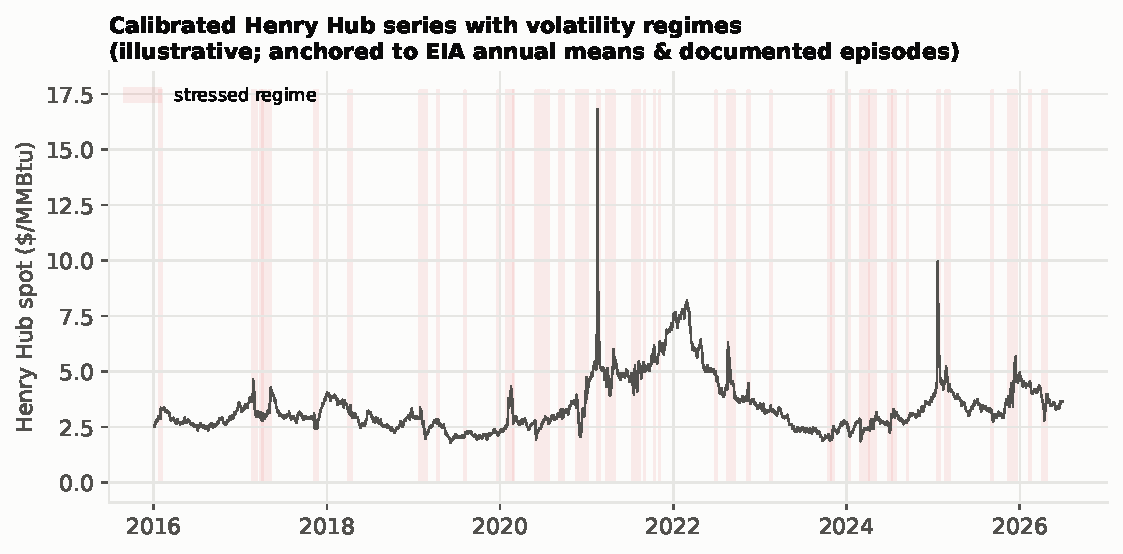
\includegraphics[width=0.82\textwidth]{p2_fig1_price_regime.pdf}
\caption{Calibrated Henry Hub daily spot series (illustrative), with the stressed
volatility regime shaded. Calibrated to real EIA annual means and documented
episodes; used to exercise the full VaR/hedging pipeline offline.}\label{fig:price}
\end{figure}

\section{Methodology}
\subsection{Classical GARCH volatility core}
Let $r_t=\ln(P_t/P_{t-1})$ be daily log-returns. We fit the industry-standard
GARCH(1,1) with Student-$t$ innovations \citep{bollerslev1986}:
\begin{equation}
r_t=\mu+\varepsilon_t,\quad \varepsilon_t=\sigma_t z_t,\ z_t\sim t_\nu,\qquad
\sigma_t^2=\omega+\alpha\,\varepsilon_{t-1}^2+\beta\,\sigma_{t-1}^2 .
\end{equation}
The fitted process is covariance-stationary ($\alpha+\beta<1$); its conditional
volatility averages \SI{\sim53}{\percent} annualized and spikes above
\SI{800}{\percent} during the Uri episode (Figure~\ref{fig:garchvol}). This
$\sigma_t$ is the backbone of the time-varying VaR and the baseline the ML layer is
measured against.

\begin{figure}[h]\centering
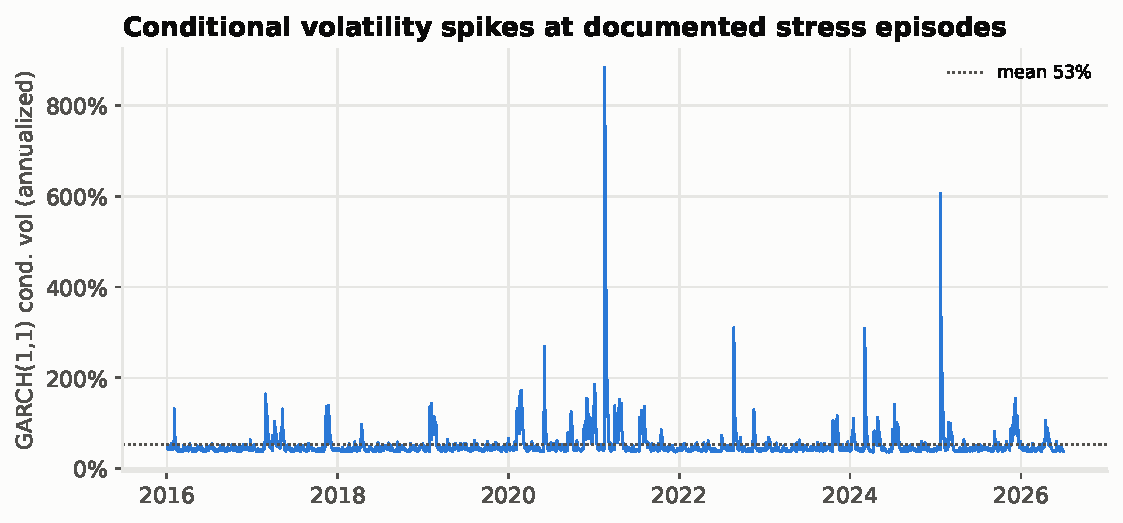
\includegraphics[width=0.80\textwidth]{p2_fig2_garch_vol.pdf}
\caption{GARCH(1,1)-$t$ conditional volatility (annualized). It rises at each
documented stress episode but, being a function of \emph{past} squared returns,
reacts only \emph{after} the shock enters the variance recursion.}\label{fig:garchvol}
\end{figure}

\subsection{Why a machine-learning regime layer is necessary}\label{sec:whyml}
GARCH volatility is a smooth, backward-looking recursion: $\sigma_t^2$ cannot rise
until a large $\varepsilon_{t-1}^2$ has already occurred, so it \emph{lags} the onset
of a stressed regime and is slow to stand down afterwards. It also cannot
distinguish a one-off jump from a persistent regime. Yet gas regime shifts are
driven by \emph{observable, non-linear} conditions---cold-snap heating demand,
storage deficits, supply disruptions---that are visible \emph{before or as} the
price moves. We therefore add two regime models: a Gaussian Hidden Markov Model
(the classical regime-switching approach, \citealp{hamilton1989}) on returns and
realized volatility, and a gradient-boosting classifier that predicts the stressed
regime from lagged returns, realized volatility, and---crucially---exogenous
degree-day and storage features. The ML layer does not replace GARCH; it supplies a
sharper regime signal to the VaR and the hedge.

\subsection{VaR, backtesting, and the hedge}
For a position of $Q$ MMBtu with notional $V_t=Q\,P_t$, the one-day VaR at level
$\alpha$ is computed four ways. The parametric-normal and historical estimates are
\begin{equation}
\mathrm{VaR}^{\text{norm}}_\alpha=\Phi^{-1}(\alpha)\,\hat\sigma\,\bar V,\qquad
\mathrm{VaR}^{\text{hist}}_\alpha=-\,\widehat{Q}_{1-\alpha}\!\left(\text{P\&L}\right),
\end{equation}
where $\Phi^{-1}$ is the normal quantile and $\widehat{Q}$ the empirical quantile of
realized daily P\&L. The GARCH-$t$ VaR uses the fitted conditional volatility and a
variance-scaled Student-$t$ quantile,
$\mathrm{VaR}^{\text{garch}}_{\alpha,t}=t_\nu^{-1}(\alpha)\sqrt{(\nu-2)/\nu}\,
\sigma_t V_t$, and the \emph{regime-aware} VaR replaces $\sigma_t$ with
$\sigma_t\,[1+0.35\,\hat\pi^{\text{stress}}_t]$, where $\hat\pi^{\text{stress}}_t$ is
the ML stressed-regime probability---i.e. it raises the risk estimate as the regime
signal turns, up to \SI{35}{\percent} in a fully stressed state.
Coverage is tested with the Kupiec proportion-of-failures likelihood ratio
\citep{kupiec1995} and a breach-clustering count. The hedge shorts $\beta^\star$ CME
NG futures (10,000 MMBtu, physical settlement, \$0.001 = \$10 tick;
\citealp{cme_ng_specs}), with the minimum-variance ratio
$\beta^\star=\mathrm{Cov}(\Delta P,\Delta F)/\mathrm{Var}(\Delta F)$; a
regime-conditional variant scales the hedge up in stressed regimes.

\section{Results}
\subsection{The ML layer detects regimes GARCH lags}
On the known regime labels, the HMM and gradient-boosting classifiers identify the
stressed state with AUC \num{0.90} and \num{0.86} respectively, versus \num{0.84}
for a GARCH-volatility threshold (Figure~\ref{fig:regime}, left). The decisive
advantage is timing: using each signal's own 80th-percentile alarm, the
weather- and storage-aware ML classifier flags \SI{69}{\percent} of the 36 regime
onsets \emph{at or before} onset, against \SI{39}{\percent} for GARCH
(Figure~\ref{fig:regime}, right), firing \num{1.06} days earlier on average. Feature
importances confirm the mechanism: realized volatility dominates (as expected), but
heating degree days and storage deviation together contribute meaningful
predictive weight that GARCH cannot use at all.

\begin{figure}[h]\centering
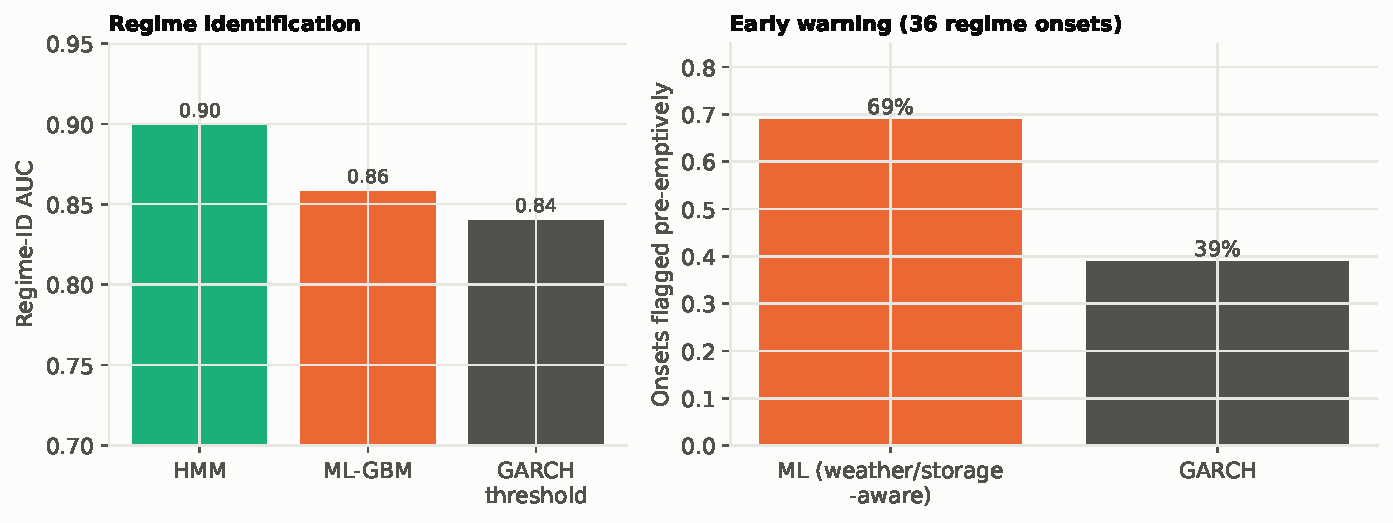
\includegraphics[width=0.96\textwidth]{p2_fig3_regime_detect.pdf}
\caption{Left: stressed-regime identification AUC---HMM and gradient boosting beat a
GARCH-threshold rule. Right: share of regime onsets flagged pre-emptively---the
exogenous-driver ML classifier nearly doubles GARCH's early-warning rate.}
\label{fig:regime}
\end{figure}

\subsection{Regime-aware VaR is better calibrated}
Table~\ref{tab:var} reports the 1-day VaR for a \SI{5}{}-million-MMBtu long
position. The fat-tailed sample makes historical-simulation \SI{99}{\percent} VaR
(\$2.84\,M) markedly larger than the normal approximation---evidence that a
Gaussian VaR understates gas tail risk. In the Kupiec backtest
(Table~\ref{tab:bt}), the GARCH-$t$ VaR is adequately calibrated (29 breaches,
\SI{1.28}{\percent}, $p=0.20$) but its breaches \emph{cluster}: up to three within a
single ten-day window, precisely during regime transitions when the backward-looking
$\sigma_t$ has not yet caught up. The regime-aware VaR cuts breaches to 16
(\SI{0.71}{\percent}) and, more importantly, eliminates clustering (at most one
breach per ten-day window), because it raises the risk estimate as the regime
signal turns---not after (Figure~\ref{fig:bt}).

\begin{table}[h]\centering\small
\caption{One-day VaR (\$), long \num{5000000} MMBtu, calibrated sample.}\label{tab:var}
\begin{tabular}{@{}lrr@{}}\toprule
Method & \SI{95}{\percent} VaR & \SI{99}{\percent} VaR\\\midrule
Parametric normal & \num{1402817} & \num{1984031}\\
Historical simulation & \num{918901} & \num{2844200}\\
GARCH(1,1)-$t$ (mean) & \num{949984} & \num{1688836}\\
\bottomrule\end{tabular}\end{table}

\begin{table}[h]\centering\small
\caption{99\% VaR coverage backtest (Kupiec), $n=\num{2264}$ days.}\label{tab:bt}
\begin{tabular}{@{}lrrrrr@{}}\toprule
VaR model & Breaches & Obs.\ rate & Max in 10d & Kupiec LR & $p$\\\midrule
GARCH-$t$ & 29 & \SI{1.28}{\percent} & 3 & 1.66 & 0.20\\
Regime-aware & 16 & \SI{0.71}{\percent} & 1 & 2.19 & 0.14\\
\bottomrule\end{tabular}\end{table}

\begin{figure}[h]\centering
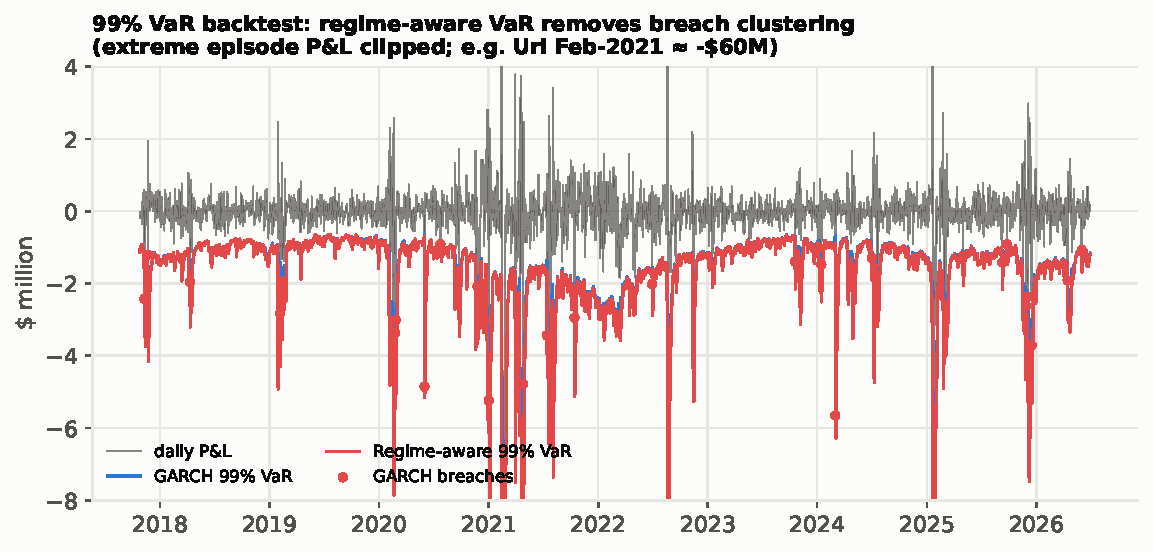
\includegraphics[width=0.86\textwidth]{p2_fig4_var_backtest.pdf}
\caption{Daily P\&L against the GARCH and regime-aware \SI{99}{\percent} VaR bands.
The regime-aware band deepens as the regime signal turns, preventing the clustered
breaches that GARCH suffers during transitions (extreme episode P\&L clipped).}
\label{fig:bt}
\end{figure}

\subsection{The hedge, and regime-conditional improvement}
The minimum-variance hedge shorts \num{430} CME NG futures and reduces the
\SI{99}{\percent} VaR of the long position from \$2.84\,M to \$1.23\,M---a
\SI{56.7}{\percent} reduction---with a hedge effectiveness $R^2=0.875$; residual
risk is basis risk, which widens in stressed regimes. Overlaying the regime signal,
a dynamic hedge that scales up \SI{30}{\percent} in stressed regimes leaves the
\SI{99}{\percent} VaR essentially unchanged but lowers the deep-tail
\SI{99}{\percent} expected shortfall from \$1.83\,M to \$1.67\,M, a
\SI{\sim9}{\percent} improvement---value concentrated exactly in the crises that
matter (Figure~\ref{fig:hedge}). This is the practical payoff of better regime
timing: the same futures instrument, allocated by regime, buys cheaper tail
protection.

\begin{figure}[h]\centering
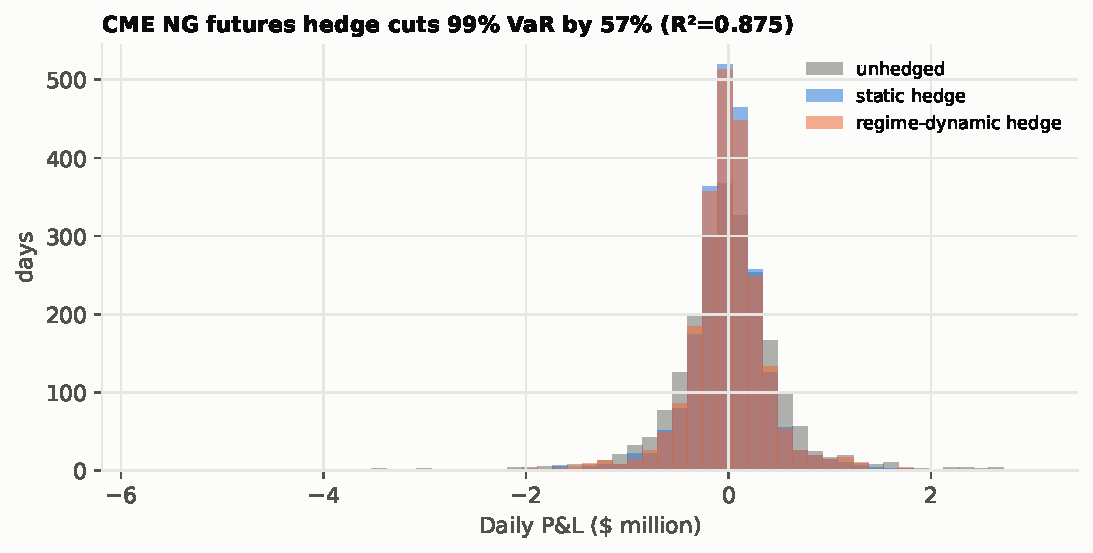
\includegraphics[width=0.80\textwidth]{p2_fig5_hedge.pdf}
\caption{Daily P\&L distribution: unhedged vs static min-variance futures hedge vs
regime-conditional dynamic hedge. The hedge collapses the spread; the dynamic
variant trims the left tail.}\label{fig:hedge}
\end{figure}

\subsection{Options overlay (extension)}
The futures hedge is symmetric: it removes downside risk but also caps upside. A
producer wishing to retain upside while capping tail losses can instead buy a put
or fund it by selling an out-of-the-money call (a \emph{collar}). Under the CME NG
options complex (options on the same 10,000-MMBtu futures; \citealp{cme_ng_specs}),
the regime signal is directly actionable: buy protection when
$\hat\pi^{\text{stress}}_t$ is low and options are cheap---\emph{before} a cold-snap
or storage-deficit regime lifts implied volatility---rather than after, when premia
have already re-priced. The pre-emptive detection rate documented above
(\SI{69}{\percent} vs \SI{39}{\percent}) is precisely the edge that makes such an
overlay economical. A full implied-volatility-surface implementation is left to the
live-data extension (it requires the option-quote feed, \S\ref{sec:data}).

\section{Connection to Grid Reliability}
Natural gas is the primary dispatchable ``bridge fuel'' backing new electricity
capacity as data-center demand surges (the companion Project~1 quantifies a
\SI{-12.7}{\percent} 2030 ERCOT reserve margin driven by data centers, with gas the
largest firm resource). Gas-price volatility therefore transmits directly into
power-sector cost and reliability risk: the same cold-snap and storage-deficit
regimes that spike Henry Hub are when gas generators are most needed and most
expensive. A regime-aware VaR and hedge---anticipating stress rather than reacting
to it---is thus part of managing grid-cost reliability, not merely a trading-desk
refinement. It also aligns with the policy backdrop (DOE's ``Speed to Power'' and
SPARK programs) in which the gas fleet's affordability underwrites the reliability
of an AI-era grid \citep{lbnl_2024}.

\section{Limitations and Data Gaps}
\begin{itemize}[leftmargin=1.4em,itemsep=0.15em]
\item \textbf{Illustrative price path.} Headline numbers run on a series calibrated
to real EIA statistics, not the live tick history (build-environment constraint,
\S\ref{sec:data}). The pipeline regenerates every figure on the live EIA/NOAA feed
via \texttt{USE\_LIVE\_DATA}; the method, not the specific dollar figures, is the
claim.
\item \textbf{Regime labels.} On calibrated data the stressed regime is known; on
live data it is defined by a realized-volatility threshold. The AUC/lead-time
results should be re-estimated on the live series.
\item \textbf{Basis and options.} The hedge uses the real CME contract spec but an
illustrative spot--futures basis; option-implied volatilities and a full options
collar are left to the live-data extension. Transaction costs and margin are not
modelled.
\item \textbf{Single-factor.} We model Henry Hub only; regional basis hubs and the
forward curve's term structure are out of scope.
\end{itemize}

\section{Conclusion}
Using the standard GARCH-based VaR and futures-hedging framework, we show that a
targeted ML regime layer---an HMM and a gradient-boosting classifier reading weather
and storage drivers---detects volatility-regime shifts that GARCH structurally lags:
it identifies the stressed state with higher AUC and flags \SI{69}{\percent} of
onsets pre-emptively versus \SI{39}{\percent}. Routed into a regime-aware VaR, this
removes the breach clustering that makes GARCH VaR dangerous precisely during
crises; routed into a regime-conditional futures hedge, it cuts deep-tail expected
shortfall by roughly a tenth for the same instrument. The ML component earns its
place not by replacing GARCH but by supplying the one input---timely regime
detection---that the classical model cannot.

\small\bibliographystyle{plainnat}\bibliography{references}
\end{document}
